\lab{Line Search Algorithms}{Line Search Algorithms}
\label{lab:line_search}
\objective{Investigate various Line-Search algorithms for numerical optimization.}

\section*{Overview of Line Search Algorithms}
Imagine you are out hiking on a mountain, and you lose track of the trail. Thick fog
gathers around, reducing visibility to just a couple of feet. You decide it is time
to head back home, which is located in the valley located near the base of the mountain.
How can you find your way back with such limited visibility? The obvious way might be to
pick a direction that leads downhill, and follow that direction as far as you can, or
until it starts leading upward again. Then you might choose another downhill direction,
and take that as far as you can, repeating the process. By always choosing a downhill
direction, you hope to eventually make it back to the bottom of the valley, where you live.

This is the basic approach of line search algorithms for numerical optimization.
Suppose we have a real-valued function $f$ that we wish to minimize. Our goal is to find the
point $x^*$ in the domain of $f$ such that $f(x^*)$ is the smallest value in the range of
$f$. For some functions, we can use techniques from calculus to analytically obtain this
minimizer. However, in practical applications, this is often impossible, especially when
we need a system that works for a wide class of functions. A line search algorithm starts with
an initial guess at the minimizer, call it $x_0$, and iteratively produces a sequence of
points $x_1, x_2, x_3, \ldots$ that hopefully converge to the minimizer $x^*$. The basic
iteration to move from $x_k$ to $x_{k+1}$ involves two steps: first, choosing a search direction $p_k$
in which to proceed from the current point, and second, specifying a step size $\alpha_k$ to travel
in this direction. The next point is determined by the formula
$$
x_{k+1} = x_k + \alpha_kp_k.
$$
This procedure is called a line search because at each iteration, we are simply examining the
function in a particular linear direction. The choice of the step size $\alpha_k$ is often
chosen by solving a one-dimensional optimization problem in the given direction. In this lab,
we will discuss approaches to choosing the step size and the search direction.

%Line search procedures are an integral part of many nonlinear optimization techniques.
%In some sense, they represent the simplest nontrivial case in general optimization, as
%we only have to worry about one parameter. And yet far more sophisticated optimization
%algorithms really crucially on the effectiveness and efficiency of line searches, since
%higher-dimensional problems are often broken down into one-dimensional optimizations.
%There are many different line search methods, and their effectiveness depends very much
%on the nature of the optimization problem. Although the line search procedure is often
%only a subroutine of the optimization algorithm at hand, understanding the basics of
%the line search is necessary for understanding the robustness of the entire algorithm.
%\section*{Optimizing Functions on the Real Numbers}
%\subsection*{Derivative versus Derivative-Free Methods}
%As you have seen in calculus classes, the derivative of a function gives information
%about how the value of the function changes at each point, and can be used to determine
%local optima. However, not all objective functions are differentiable, so we need other
%techniques at our disposal. Line search methods may be broadly separated into two groups
%based on whether they use the derivative of the objective function. We discuss two
%simple examples to illustrate this distinction.
%
%\subsection*{Golden Section Search}
%This method is appropriate when minimizing a real-valued function on the reals over a
%closed interval. The function must further satisfy the \emph{unimodal} property, i.e.
%it has just one local minimum, and is monotonic to the left and right of the minimum.
%The goal, of course, is to find the
%global minimum. We do this by making a sequence of guesses that we hope will converge
%quickly to the minimum. Although we may not end up with the exact minimum, this method
%will allow us to pin down the true minimum within an interval of any given width in a
%finite number of steps.
%
%For the Golden Section Search, each step consists of evaluating the function at two
%points within the current interval, comparing these values, and then reducing the size
%of the interval for the next step. Let us consider a typical step in the algorithm. At
%the outset, we have our function $f$ and a closed interval $[a, b]$ over which we seek
%to minimize $f$. Choose two points $a'$ and $b'$ within the interval, and assume that
%$a' < b'$. Now calculate $f(a')$ and $f(b')$, and assume that $f(a') \geq f(b')$.
%Because of the unimodal condition, we now know that the minimizer must be in the
%interval $[a', b]$, for otherwise the function $f$ would have a local minimum in
%both $[a, a']$ and $[a', b]$. In the next step, we repeat the process over the interval
%$[a', b]$. If instead we had $f(b') \geq f(a')$, then we choose the interval $[a, b']$
%for the next step, and if the two values are equal, then it does not matter which
%interval is chosen.
%
%We now have the basic description of the algorithm, but how do we choose the two test
%points $a'$ and $b'$? There is in fact an optimal choice, which reduces the amount of
%work we have to do. Given an interval $[a, b]$, choose $a'$ and $b'$ satisfying
%\begin{align*}
%a' &= a + \rho(b - a) \\
%b' &= a + (1 - \rho)(b - a),
%\end{align*}
%where $\rho = \frac{1}{2}(3 - \sqrt{5}) \approx 0.382$. By choosing these particular
%points, we need to only evaluate the function at one additional point in the next step.
%To demonstrate this fact, the reader may verify that, within the interval $[a, b']$,
%the point $a'$ already satisfies the equation
%\begin{equation*}
%a' = a + (1 - \rho)(b' - a),
%\end{equation*}
%and so we need only evaluate the function at the point $c$ satisfying
%\begin{equation*}
%c = a + \rho(b' - a).
%\end{equation*}
%(The constant $\rho$ is not difficult to derive, and is related to the famous Golden Ratio, hence the name of this algorithm.)
%
%At each step, the interval is reduced by a factor of $1-\rho$, which means that after
%$n$ steps, we have pinned down the minimizer to within an interval approximately
%$(0.61803)^n$ times the length of the original interval. Note that this convergence is
%independent of the objective function.
%
%\begin{problem}
%Implement Golden Section Search as described above. Use this to minimize $e^x - 4x$
%on the interval $\lbrack 0, 3 \rbrack$. How many steps do you need to take to get
%within $.001$ of the true minimizer? Check that with the sentence preceding this
%problem.
%\end{problem}

\subsection*{One-Dimensional Newton's Method}
Let us first start out with a basic task: minimizing a function of one variable.
We will use a popular approach known as Newton's Method, which is a basic line search
algorithm that uses the derivatives of the function to select a direction and
step size.

To use this method, we need a real-valued function of a real variable that is twice
differentiable. The idea is to approximate the function with a quadratic polynomial and
then solve the trivial problem of minimizing the polynomial. Doing so in an iterative
manner can lead us to the actual minimizer. Let $f$ be a function satisfying the
appropriate conditions, and let us make an initial guess, $x_0$. The relevant quadratic
approximation to $f$ is
\begin{equation*}
q(x) = f(x_0) + f'(x_0)(x-x_0) + \frac{1}{2}f''(x_0)(x-x_0)^2,
\end{equation*}
or just the second-degree Taylor polynomial for $f$ centered at $x_0$. The minimum
for this quadratic function is easily found by solving $q'(x) = 0$, and we take the
obtained $x$-value as our new approximation. The formula for the $(n+1)$-th
approximation, which the reader can verify, is
\begin{equation*}
x_{n+1} = x_n - \frac{f'(x_n)}{f''(x_n)}.
\end{equation*}

As is typical with optimization algorithms, Newton's Method generates a sequence of
points or successive approximations to the minimizer. However, the convergence
properties of this sequence depend heavily on the initial guess $x_0$ and the function
$f$. Roughly speaking, if $x_0$ is sufficiently close to the actual minimizer, and if
$f$ is well-approximated by parabolas, then one can expect the sequence to converge
quickly. However, there are cases when the sequence converges slowly or not at all.
See Figure \ref{linesearch:newton}.

\begin{figure}
\centering
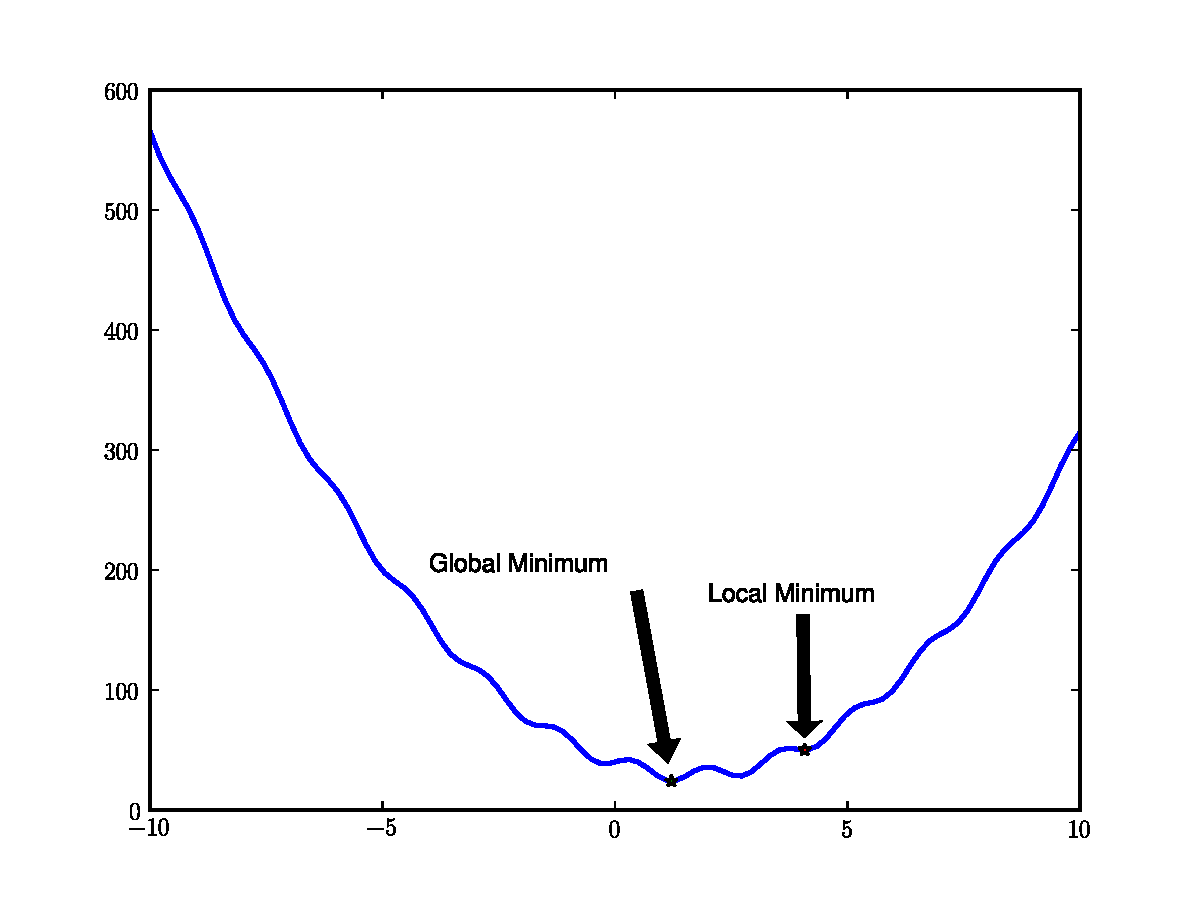
\includegraphics[width=\textwidth]{newton.pdf}
\caption{The results of Newton's Method using two
different initial guess. The global minimizer was
correctly found with initial guess of 1. However,
an initial guess of 4 led to only a local minimum.}
\label{linesearch:newton}
\end{figure}

\begin{problem}
Implement Newton's Method as described above. Write a function called \li{newton1d} that
accepts a function object for the objective function, the first derivative, and the
second derivative, a real number giving the initial point, and an integer giving the number
of iterations. The function should perform Newton's method for the specified number of iterations
and return the approximated minimizer.

Use this function to minimize $x^2 + \sin(5x)$ with an initial guess of $x_0 = 0$.
Now try other initial guesses farther away from the true minimizer, and note when the
method fails to obtain the correct answer.
\end{problem}

\section*{General Line Search Methods}
\subsection*{Step Size Calculation}
We now examine Line Search methods in more generality. Given a differentiable function
$f : \mathbb{R}^n \rightarrow \mathbb{R}$ that we wish to minimize, and assuming that
we already have a current point $x_k$ and direction $p_k$ in which to search, how do we
choose our step size $\alpha_k$? If our step size is too small, we will not make good progress
toward the minimizer, and convergence will be slow. If the step size is too large, however,
we may overshoot and produce points that are far away from the solution.
A common approach to pick an appropriate step size involves the \emph{Wolfe conditions}:

\begin{align*}
&f(x_k + \alpha_kp_k) \leq f(x_k) + c_1\alpha_k\nabla f_k^Tp_k, &(0 < c_1 < 1),
\\ &\nabla f(x_k + \alpha_kp_k)^Tp_k \geq c_2\nabla f_k^Tp_k, &(c_1 < c_2 < 1).
\end{align*}

Here, we use the shorthand notation $\nabla f_k$ to
mean the gradient of $f$ evaluated at the point $x_k$. The search direction $p_k$ is
often required to satisfy $p_k^T \nabla f_k < 0$, in which case it is called a
\emph{descent direction}, since the function is guaranteed to decrease in
this direction. Generally speaking, choosing a step size $\alpha_k$ satisfying these conditions
ensures that we achieve sufficient decrease in the function and also that we do not
terminate the search at a point of steep decrease (since then we could achieve even
better results by choosing a slightly larger step size). The first condition is known
as the \emph{Armijo} condition.

Finding such a step size satisfying these conditions is not always an easy task, however.
One simple approach, known as \emph{backtracking}, starts with an initial step size
$\alpha$, and repeatedly scales it down until the Armijo condition is satisfied.
That is, choose $\alpha >0, \rho \in (0, 1), c\in (0, 1)$, and while
$$
f(x_k + \alpha p_k) > f(x_k) + c\alpha\nabla f_k^Tp_k,
$$
set $\alpha := \rho\alpha$. Once the loop terminates, set $\alpha_k = \alpha$. Note that the value
$\nabla f_k^Tp_k$ remains fixed for the duration of the backtracking algorithm, and hence need only
be calculated once at the beginning.
%The second of the two conditions can be replaced by
%\begin{equation*}
%| \nabla f(x_k + \alpha_kp_k)^Tp_k| \leq c_2 | \nabla f_k^Tp_k|,
%\end{equation*}
%and in this case we have the \emph{strong Wolfe conditions}.
%
%The \emph{Goldstein conditions} for choosing step size:
%\begin{equation*}
%f(x_k) + (1-c)\alpha_k\nabla f_k^Tp_k \leq f(x_k + \alpha_kp_k) \leq f(x_k) +
%c\alpha_k\nabla f_k^Tp_k,
%\end{equation*}
%where $0 < c < 0.5$. Similar to the Wolfe conditions, the Goldstein conditions ensure
%sufficient decrease in the function and prevent the step size from being too small. In
%the area of quasi-Newton optimization methods, however, the Wolfe conditions are
%preferred.

\begin{problem}
Implement this backtracking algorithm. Write a function \li{backtrack} that takes a function
object giving the objective function, a real number giving the value of $\nabla f_k^Tp_k$, the
current point $x_k$, the search direction $p_k$, an initial guess for $\alpha$, the value for
$\rho$, and the value for $c$. Return the computed step size.
\end{problem}

\subsection*{Choosing a Search Direction}
There are many different ways to choose a search direction $p_k$. As noted earlier, it is usually
a requirement to choose a descent direction. We will compare two methods, both using derivative
information about the function.

\emph{Gradient Descent.} Recall that the gradient of a function at a given point gives the direction
in which the function is increasing fastest. Thus, the negative of the gradient points in the direction
of fastest decrease. In the method of Gradient Descent, we choose our search direction to be
this direction of steepest descent, that is,
$$
p_k = -\nabla f_k.
$$
This is a very natural choice, since we seem to be approaching the minimum value as fast as possible.
However, depending on the nature of the objective function, convergence may be slow. See Figure
\ref{linesearch:comparison}.

\begin{figure}
\centering
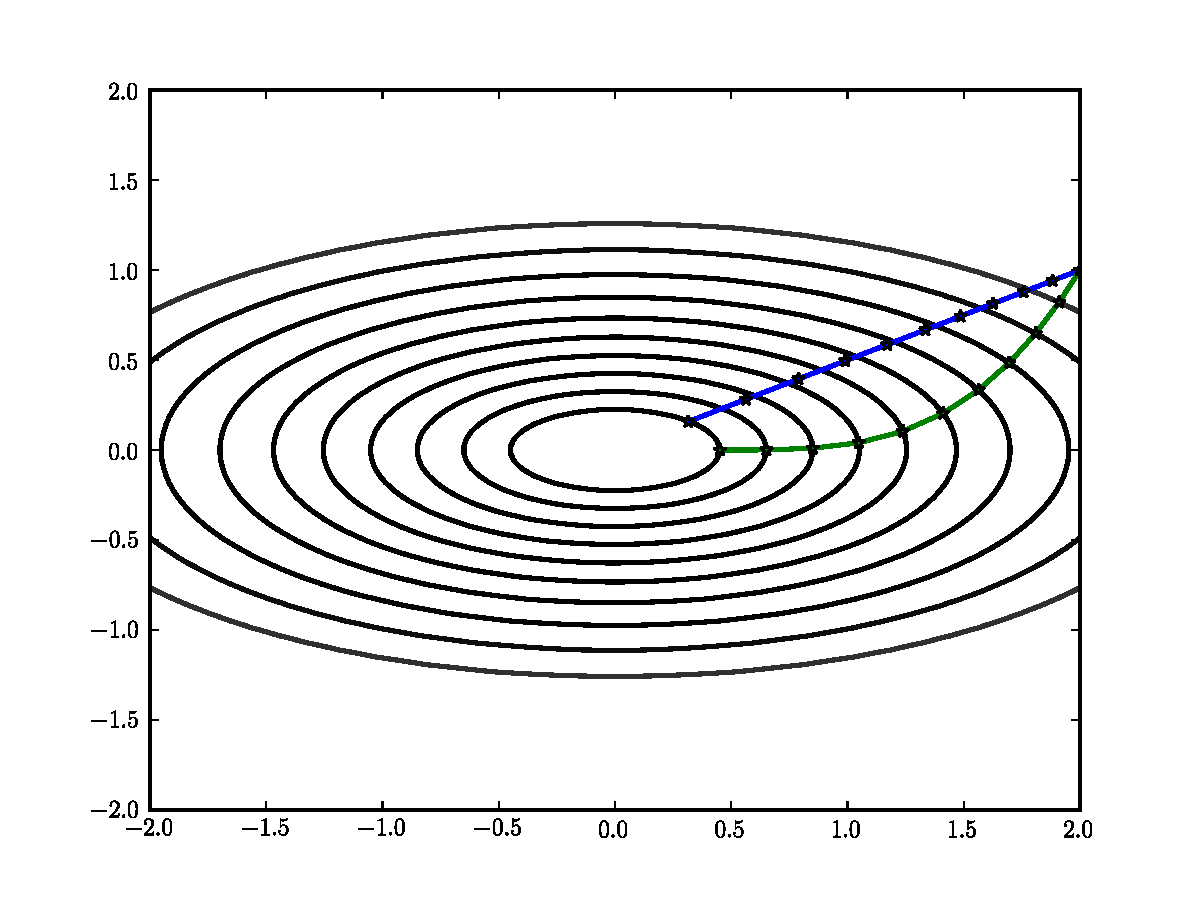
\includegraphics[width=\textwidth]{comparison.pdf}
\caption{Paths generated by Gradient Descent (green) and Newton's Method (blue).
Note that the Newton path takes a more direct route toward the minimizer (located
at the origin).
}
\label{linesearch:comparison}
\end{figure}

\emph{Newton's Method.} We now generalize the one-dimensional Newton's method presented above.
We use both the gradient and the Hessian matrix (which gives information on the curvature of the
function at a given point) to choose a search direction. This is more computationally intensive,
but it leads to very fast convergence in many cases. See Figure
\ref{linesearch:comparison}. Our search direction is
$$
p_k = -\nabla^2 f_k^{-1} \nabla f_k,
$$
where $\nabla^2 f_k^{-1}$ is the inverse of the Hessian matrix of $f$ at the point $x_k$.
In other words, $p_k$ is the solution to the linear system
$$
\nabla^2 f_k p_k = -\nabla f_k.
$$

\begin{problem}
Write a function \li{gradientDescent} that implements the Gradient Descent algorithm.
Write another function \li{newtonsMethod} that implements the general Newton's Method
described above. In each function, you should call your backtracking function with
values $\alpha = 1, \rho = .9$, and $c = 10^{-4}$. The \li{scipy.linalg} module
may be useful when computing the search direction in Newton's Method.
\end{problem}

\subsection*{Line Search in SciPy}
The SciPy module \li{scipy.optimize} contains implementations of various optimization algorithms,
including several line search methods. In particular, the module provides a useful routine for
calculating a step size satisfying the Wolfe Conditions described above, which is more robust
and efficient than our simple backtracking approach. We recommend its use for the remainder of
this lab. The function is called \li{line_search}, and accepts several arguments. We can typically
leave the keyword arguments at their default values, but we do need to pass in the objective
function, its gradient, the current point, and the search direction. The following code gives
an example of its usage, using the objective function $f(x, y) = x^2+4y^2$.
\begin{lstlisting}
>>> import numpy as np
>>> from scipy.optimize import line_search
>>>
>>> def objective(x):
>>>     return x[0]**2 + 4*x[1]**2
>>>
>>> def grad(x):
>>>     return 2*x*np.array([1, 4])
>>>
>>> x = np.array([1., 3.]) #current point
>>> p = -grad(x)           #current search direction
>>> a = line_search(objective, grad, x, p)[0]
>>> print a
0.125649913345
\end{lstlisting}
Note that the function returns a tuple of values, the first of which is the step size. We have illustrated
the very basic use of this function. See the documentation for further uses.

\section*{Non-linear Least Squares Problems}
We now discuss a very important class of problems known as Least Squares problems. These
are unconstrained optimization problems that seek to minimize an objective function of the form
$$
f(x) = \frac{1}{2}\displaystyle\sum_{j=1}^m r_j^2(x),
$$
where each $r_i : \mathbb{R}^n \rightarrow \mathbb{R}$ is smooth, and $m \geq n$. Such problems
arise in many scientific fields, including economics, physics, and statistics. Linear Least
Squares problems form an important subclass, and can be solved directly without the need for an
iterative method. At present we will focus on the non-linear case, which can be solved with a
line search method.

To motivate the problem further, suppose you are given a set of data points, and you have some kind of model for the data.
You need to choose particular values for the parameters in your model, and you wish to do so in a way that ``best fits"
the observed data. What do we mean by ``best fit"? We need some way to measure the error between our model and the data set,
and then minimize this error. The best fit will correspond to the choice of parameters that minimize the error function.

More formally, suppose we are given the data points $(t_1, y_1), (t_2, y_2), \ldots, (t_m, y_m)$, where $y_i \in \mathbb{R}$
and $t_i \in \mathbb{R}^n$ for $i = 1, \ldots, m$. Let $\phi(x, t)$ be our model for this data set, where $x$ is
a vector of parameters of the model, and $t \in \mathbb{R}^n$. We can measure the error at the $i$-th data point by the value
$$r_i(x) := \phi(x, t_i) - y_i,$$ and by summing the squares of these errors, we obtain our non-linear least squares objective
function:
$$
f(x) = \frac{1}{2} \displaystyle \sum_{j=1}^m  r_j^2(x).
$$

The individual functions $r_i$ that measure the error between the model and the data point are known as \emph{residuals},
and we can aggregate these functions into a \emph{residual vector}
$$
r(x) := (r_1(x), r_2(x), \ldots, r_m(x))^T.
$$
The Jacobian of $r(x)$ can be expressed in terms of the gradients of each $r_i$ as follows:
$$
J(x) = \begin{bmatrix} \nabla r_1(x)^T \\ \nabla r_2(x)^T \\ \vdots \\ \nabla r_m(x)^T \end{bmatrix}
$$
You can further verify that
\begin{align*}
\nabla f(x) &= J(x)^T r(x), \\
\nabla^2 f(x) &= J(x)^TJ(x) + \displaystyle \sum_{j=1}^m r_j(x) \nabla^2r_j(x).
\end{align*}
That second term in the formula for $\nabla^2 f$ involves second derivatives and can be problematic to compute. Often in practice,
this term is small, either because the residuals themselves are small, or are nearly affine in a neighborhood of the solution and
hence the second derivatives are small.
The simplest method for solving the nonlinear least squares problem, known as the \emph{Gauss-Newton Method}, exploits this
observation, simply ignoring the second term and making the approximation
$$
\nabla^2 f(x) \approx J(x)^TJ(x).
$$
The method then proceeds in a manner similar to Newton's Method. In particular, at the $k$-th iteration, we choose a search
direction $p_k$ that solves the linear system
$$
J_k^TJ_kp_k = -J_k^Tr_k.
$$

For convenience, we summarize these steps in Algorithm \ref{alg:guassnewton}.
\begin{algorithm}
\begin{algorithmic}[1]
\Procedure{Gauss-Newton}{}
    \State \textrm{Choose initial parameter vector } $x_0$
    \State $k \gets 0$
    \While{$J_k^Tr_k \neq 0$}
        \State \textrm{solve } $J_k^TJ_kp_k = -J_k^Tr_k$
        \State \textrm{choose step size } $\alpha_k$ \textrm{ satisfying Wolfe Conditions.}
        \State $x_{k+1} \gets x_k + \alpha_kp_k$
        \State $k \gets k+1$
    \EndWhile
\EndProcedure
\end{algorithmic}
\caption{Gauss-Newton Method}
\label{alg:guassnewton}
\end{algorithm}

\begin{problem}
Write a function called \li{gaussNewton} that implements the algorithm described above.
The function should take functions objects for the objective function, its gradient, the Jacobian,
the residual vector, an initial guess, and a number of iterations. It should return the estimated
parameters.

Feel free to use SciPy functions to solve linear systems and calculate step sizes in your algorithm.
\end{problem}

Let us work through an example of a nonlinear least squares problem. Suppose we have data points
generated from a sine function and slightly perturbed by gaussian noise. In Python we can generate such
data as follows:
\begin{lstlisting}
>>> t = np.arange(10)
>>> y = 3*np.sin(0.5*t)+ 0.5*np.random.randn(10)
\end{lstlisting}
Now we write Python functions for our model, the residual vector, the Jacobian, the objective function,
and the gradient. The calculations for all of these are straight forward.
\begin{lstlisting}
>>> def model(x, t):
>>>     return x[0]*np.sin(x[1]*t)
>>> def residual(x):
>>>     return model(x, t) - y
>>> def jac(x):
>>>     ans = np.empty((10,2))
>>>     ans[:,0] = np.sin(x[1]*t)
>>>     ans[:,1] = x[0]*t*np.cos(x[1]*t)
>>>     return ans
>>> def objective(x):
>>>     return .5*(residual(x)**2).sum()
>>> def grad(x):
>>>     return jac(x).T.dot(residual(x))
\end{lstlisting}
By inspecting our data, we might make an initial guess for the parameters $x_0 = (2.5, 0.6)$.
We are now ready to use our \li{gaussNewton} function to find the least squares solution.
\begin{lstlisting}
>>> x0 = np.array([2.5,.6])
>>> x = gaussNewton(objective, grad, jac, residual, x0, niter=10)
\end{lstlisting}
We can plot everything together to compare our fitted model with the data and the original sine
curve from which the data were generated.
\begin{lstlisting}
dom = np.linspace(0,10,100)
plt.plot(t, y, '*')
plt.plot(dom, 3*np.sin(.5*dom), '--')
plt.plot(dom, x[0]*np.sin(x[1]*dom))
plt.show()
\end{lstlisting}
The results are shown in Figure \ref{linesearch:gaussNewton}. As you can see, after just 10
iterations, we have found a very good fit.
\begin{figure}
\centering
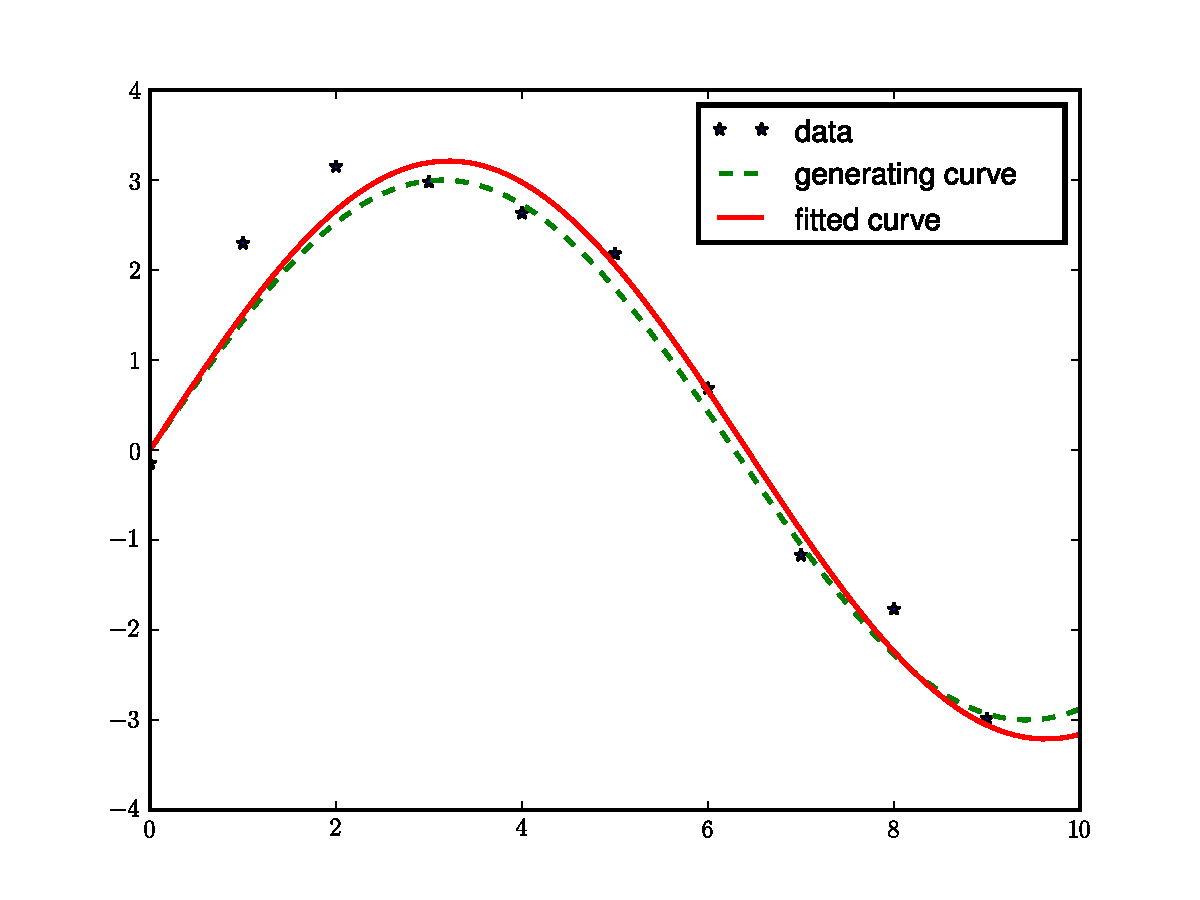
\includegraphics[width=\textwidth]{gaussNewton.pdf}
\caption{Perturbed data (stars) generated from a sine curve (dashed line),
together with the fitted sine curve (solid line).
}
\label{linesearch:gaussNewton}
\end{figure}

\subsection*{Non-linear Least Squares in Python}
The module \li{scipy.optimize} also has a method to solve non-linear least squares problem, and it
is quite convenient. The function is called \li{leastsq}, and in its most basic use, you only need
to pass in the residual function and starting point as arguments. In the example above, we simply
need to execute the following code:
\begin{lstlisting}
>>> from scipy.optimize import leastsq
>>> x2 = leastsq(residual, x0)[0]
\end{lstlisting}
This should give us the same answer, but much faster.
\begin{problem}
We have census data giving the population of the United States every ten years since 1790.
For convenience, we have entered the data in Python below, so that you may simply copy and
paste.
\begin{lstlisting}
>>> #Start with the first 8 decades of data
>>> years1 = np.arange(8)
>>> pop1 = np.array([3.929, 5.308, 7.240, 9.638, 12.866,
>>>                 17.069, 23.192, 31.443])
>>>
>>> #Now consider the first 16 decades
>>> years2 = np.arange(16)
>>> pop2 = np.array([3.929, 5.308, 7.240, 9.638, 12.866,
>>>                 17.069, 23.192, 31.443, 38.558, 50.156,
>>>                 62.948, 75.996, 91.972, 105.711, 122.775,
>>>                 131.669])
\end{lstlisting}
Consider just the first 8 decades of population data. By plotting the data and having
an inclination that population growth tends to be exponential, it is reasonable to
hypothesize an exponential model for the population, that is,
$$
\phi(x_1,x_2,x_3,t) = x_1\exp(x_2(t+x_3)).
$$
By inspection, find a reasonable
initial guess for the parameters $(x_1, x_2, x_3)$.
Write a function for this model in Python, along with the corresponding residual vector,
and fit the model using the \li{leastsq} function.  Plot the data against the fitted curve,
to see how close you are.

Now consider all 16 decades of data. If you plot your curve from above with this more complete
data, you will see that the model is no longer a good fit. Instead, the data suggest
a logistic model, which also arises from a differential equations treatment of population growth.
Thus, your new model is
$$
\phi(x_1,x_2,x_3,t) = \frac{x_1}{1+\exp(-x_2(t+x_3))}.
$$
By inspection, find a reasonable
initial guess for the parameters $(x_1, x_2, x_3)$.
Again, write Python functions for the model and the corresponding residual vector,
and fit the model. Plot the data against the fitted curve. It should be a good fit.
\end{problem} 